\documentclass[11pt, english, fleqn, DIV=15, headinclude, BCOR=2cm]{scrreprt}

\usepackage[
    color,
    bibatend,
]{../../header}

\graphicspath{{./}{../Figures/}}

\usepackage{needspace}

\usepackage{mathtools}
\usepackage{listings}

\lstset{
    basicstyle=\small\ttfamily,
}

\hypersetup{
    pdftitle=
}

\newcommand\mot{\textsc{mot}}

\usepackage{longtable}
\usepackage{subcaption}

\usepackage[all]{nowidow}

\subject{Lab report}
\title{Optical frequency doubling}
\subtitle{Experiment A245 -- Universität Bonn}
\author{%
    Martin Ueding \\
    \small{\href{mailto:mu@martin-ueding.de}{mu@martin-ueding.de}}
    \and
    Lino Lemmer \\
    \small{\href{mailto:l2@uni-bonn.de}{l2@uni-bonn.de}}
}

\date{\daterange{2016-05-23}{2016-05-24}}

\publishers{Tutor: Gautam Ramola}

\begin{document}

\maketitle

\begin{abstract}
\end{abstract}

\tableofcontents

\chapter*{Permission to upload}

I, Martin Ueding, would like to scan and upload this lab report with your
corrections to my website \href{http://martin-ueding.de}{martin-ueding.de}.
There, the original lab report as well as the reviewed one will be licensed
under the “\href{http://creativecommons.org/licenses/by-sa/4.0/}{Creative
Commons Attribution-ShareAlike 4.0 International License}”. Is that okay with
you?

Yes $\Box$ \hspace{2cm} No $\Box$

\chapter{Theory}


\section{Generation of hamonics}

\section{Birefringence}

\subsection{Retarder plates}

\section{Phase matching}

\section{Gaussian beams}

\section{Wavelength measurement}

\subsection{Gratings}

\subsection{Michelson interferometer}

\section{Coherence}

\subsection{Coherence length}

\section{Diode laser}

\chapter{Conduction and analysis}

\section{Diode laser classification}

\subsection{Injection current}

\subsection{Threshold current}

\subsection{Quantum efficiency}

\subsection{Attenuator}

\section{Harmonic power}

\begin{figure}
    \centering
    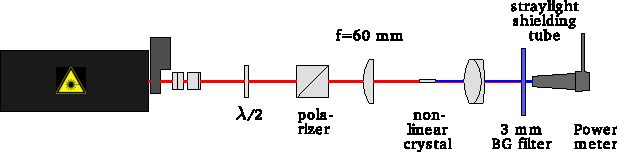
\includegraphics{fig-4}
    \caption{%
        %
    }
    \label{fig:fig-4}
\end{figure}

\subsection{Output power optimization}

\subsection{Crystal temperature dependence}

\subsection{Input power dependence}

\subsection{Input polarization dependence}

\section{Wavelength comparison}

\subsection{Grating}

\subsection{Michelson interferometer}

\begin{figure}
    \centering
    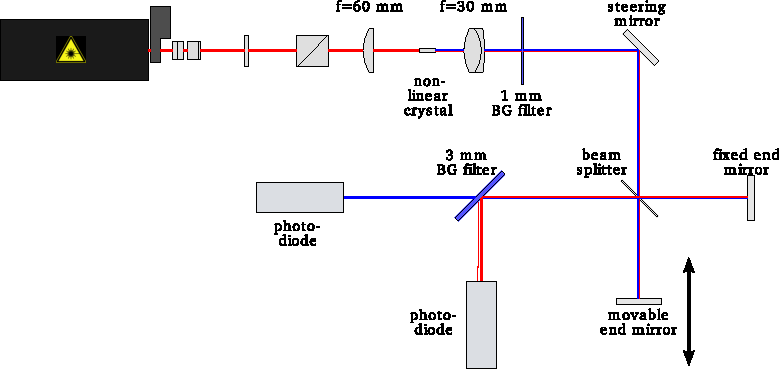
\includegraphics{fig-5}
    \caption{%
        %
    }
    \label{fig:fig-5}
\end{figure}

\end{document}

% vim: spell spelllang=en_us tw=79
